\section{Results \& Analysis}
% GOAL: Present main leaderboard, resurrection paired comparison, ranking shift, scaffold interaction.

\subsection{Main Leaderboard}

Table~\ref{tab:main} presents the full \eva{} leaderboard across 19 model configurations.

\begin{table*}[t]
\centering
\small
\resizebox{\textwidth}{!}{
\begin{tabular}{llrrrrrrrrrr}
\toprule
\textbf{Model} & \textbf{Backend} & \textbf{T0} & \textbf{T1} & \textbf{T2} & \textbf{T3} & \textbf{T4} & \textbf{T5} & \textbf{MR} & \textbf{PS} & \textbf{PL} & \textbf{Res} \\
\midrule
\underline{gpt-5.5} & codex & \textbf{100} & \textbf{100} & \textbf{100} & \textbf{100} & \textbf{95} & \textbf{100} & 98.5 & 100.0 & 99.2 & 0 \\
claude-sonnet-4.6 & claude & \textbf{100} & \textbf{100} & \textbf{100} & 98.6 & 94.6 & \textbf{100} & 98.3 & 77.8 & 98.9 & 4 \\
qwen3.6-flash & openhands & \textbf{100} & \textbf{100} & \textbf{100} & \textbf{100} & \textbf{92} & \textbf{100} & 97.5 & 66.7 & 98.6 & 2 \\
\underline{deepseek-v4-pro} & openhands & \textbf{100} & \textbf{100} & \textbf{100} & \textbf{100} & 71 & \textbf{100} & 91.4 & 66.7 & 95.2 & 0 \\
minimax-m2.7 & openhands & \textbf{100} & 61 & \textbf{100} & \textbf{93} & \textbf{98} & \textbf{100} & 90.4 & 66.7 & 91.9 & 2 \\
qwen3.6-max-preview & openhands & \textbf{100} & 61 & \textbf{100} & \textbf{97} & \textbf{94} & \textbf{100} & 90.0 & 66.7 & 92.0 & 3 \\
glm-5 & openhands & \textbf{100} & \textbf{100} & \textbf{100} & \textbf{100} & 63 & \textbf{100} & 88.8 & 66.7 & 93.8 & 1 \\
qwen3.6-plus & openhands & \textbf{100} & \textbf{100} & 74 & 73 & \textbf{81} & \textbf{100} & 85.0 & 66.7 & 88.0 & 2 \\
deepseek-v4-flash & openhands & \textbf{100} & 0 & \textbf{100} & \textbf{93} & \textbf{90} & \textbf{100} & 75.8 & 55.6 & 80.5 & 3 \\
glm-4.7 & openhands & \textbf{100} & 0 & 62 & \textbf{100} & \textbf{94} & \textbf{100} & 70.5 & 55.6 & 75.9 & 1 \\
minimax-m2.5 & openhands & \textbf{100} & \textbf{100} & 0 & 73 & \textbf{80} & \textbf{100} & 70.0 & 55.6 & 75.5 & 2 \\
qwen3.5-plus & openhands & \textbf{100} & \textbf{100} & 0 & 53 & \textbf{87} & \textbf{100} & 69.0 & 44.4 & 73.3 & 2 \\
qwen3-coder-flash & openhands & \textbf{100} & \textbf{100} & 0 & 34 & 58 & \textbf{100} & 65.3 & 44.4 & 73.7 & 3 \\
mimo-v2.5-pro & openhands & \textbf{100} & 0 & \textbf{100} & \textbf{100} & 60 & \textbf{100} & 70.8 & 55.6 & 70.8 & 3 \\
kimi-k2-thinking & openhands & \textbf{100} & 0 & \textbf{100} & \textbf{100} & 60 & \textbf{100} & 63.5 & 55.6 & 63.5 & 2 \\
deepseek-reasoner & openhands & \textbf{100} & 0 & 21 & \textbf{100} & 60 & \textbf{100} & 63.5 & 55.6 & 63.5 & 2 \\
deepseek-chat & openhands & \textbf{100} & 0 & 21 & \textbf{100} & 60 & \textbf{100} & 63.5 & 55.6 & 63.5 & 2 \\
qwen-omni-turbo & openhands & \textbf{100} & 0 & 0 & 0 & 0 & 0 & 50.9 & 33.3 & 62.6 & 2 \\
glm-5.1 & openhands & \textbf{100} & 0 & 0 & 0 & 0 & 0 & 38.8 & 38.9 & 48.6 & 0 \\
\bottomrule
\end{tabular}}
\caption{\eva{} leaderboard across 19 model configurations. \underline{Underlined} models achieved zero-shot pipeline success (no resurrection). \textbf{Bold} scores indicate task passing ($\geq 60\%$). MR = Mean Reward, PS = Pass Score, PL = Pipeline Score, Res = Resurrection count.}
\label{tab:main}
\end{table*}

\textbf{Key observation.}
Only 2 out of 18 configurations (GPT-5.5/Codex and deepseek-v4-pro/OpenHands) achieve zero-shot pipeline success without any resurrection.
Most configurations require at least one resurrection, and several models that score well on individual tasks show significant score drops when evaluated in the serial setting---a pattern invisible to static benchmarks.

\subsection{Resurrection Recovers Hidden Downstream Capability}

Figure~\ref{fig:resurrection_gain} shows the per-task score improvement when resurrection is enabled versus the no-resurrection setting.
Without resurrection, 16 out of 19 configurations cannot reach the full pipeline depth of 6 tasks; the median zero-shot pipeline depth is only 1 task.
With resurrection, all configurations can be evaluated at every downstream node, recovering diagnostic signal that would otherwise be lost.

\begin{figure}[t]
\centering
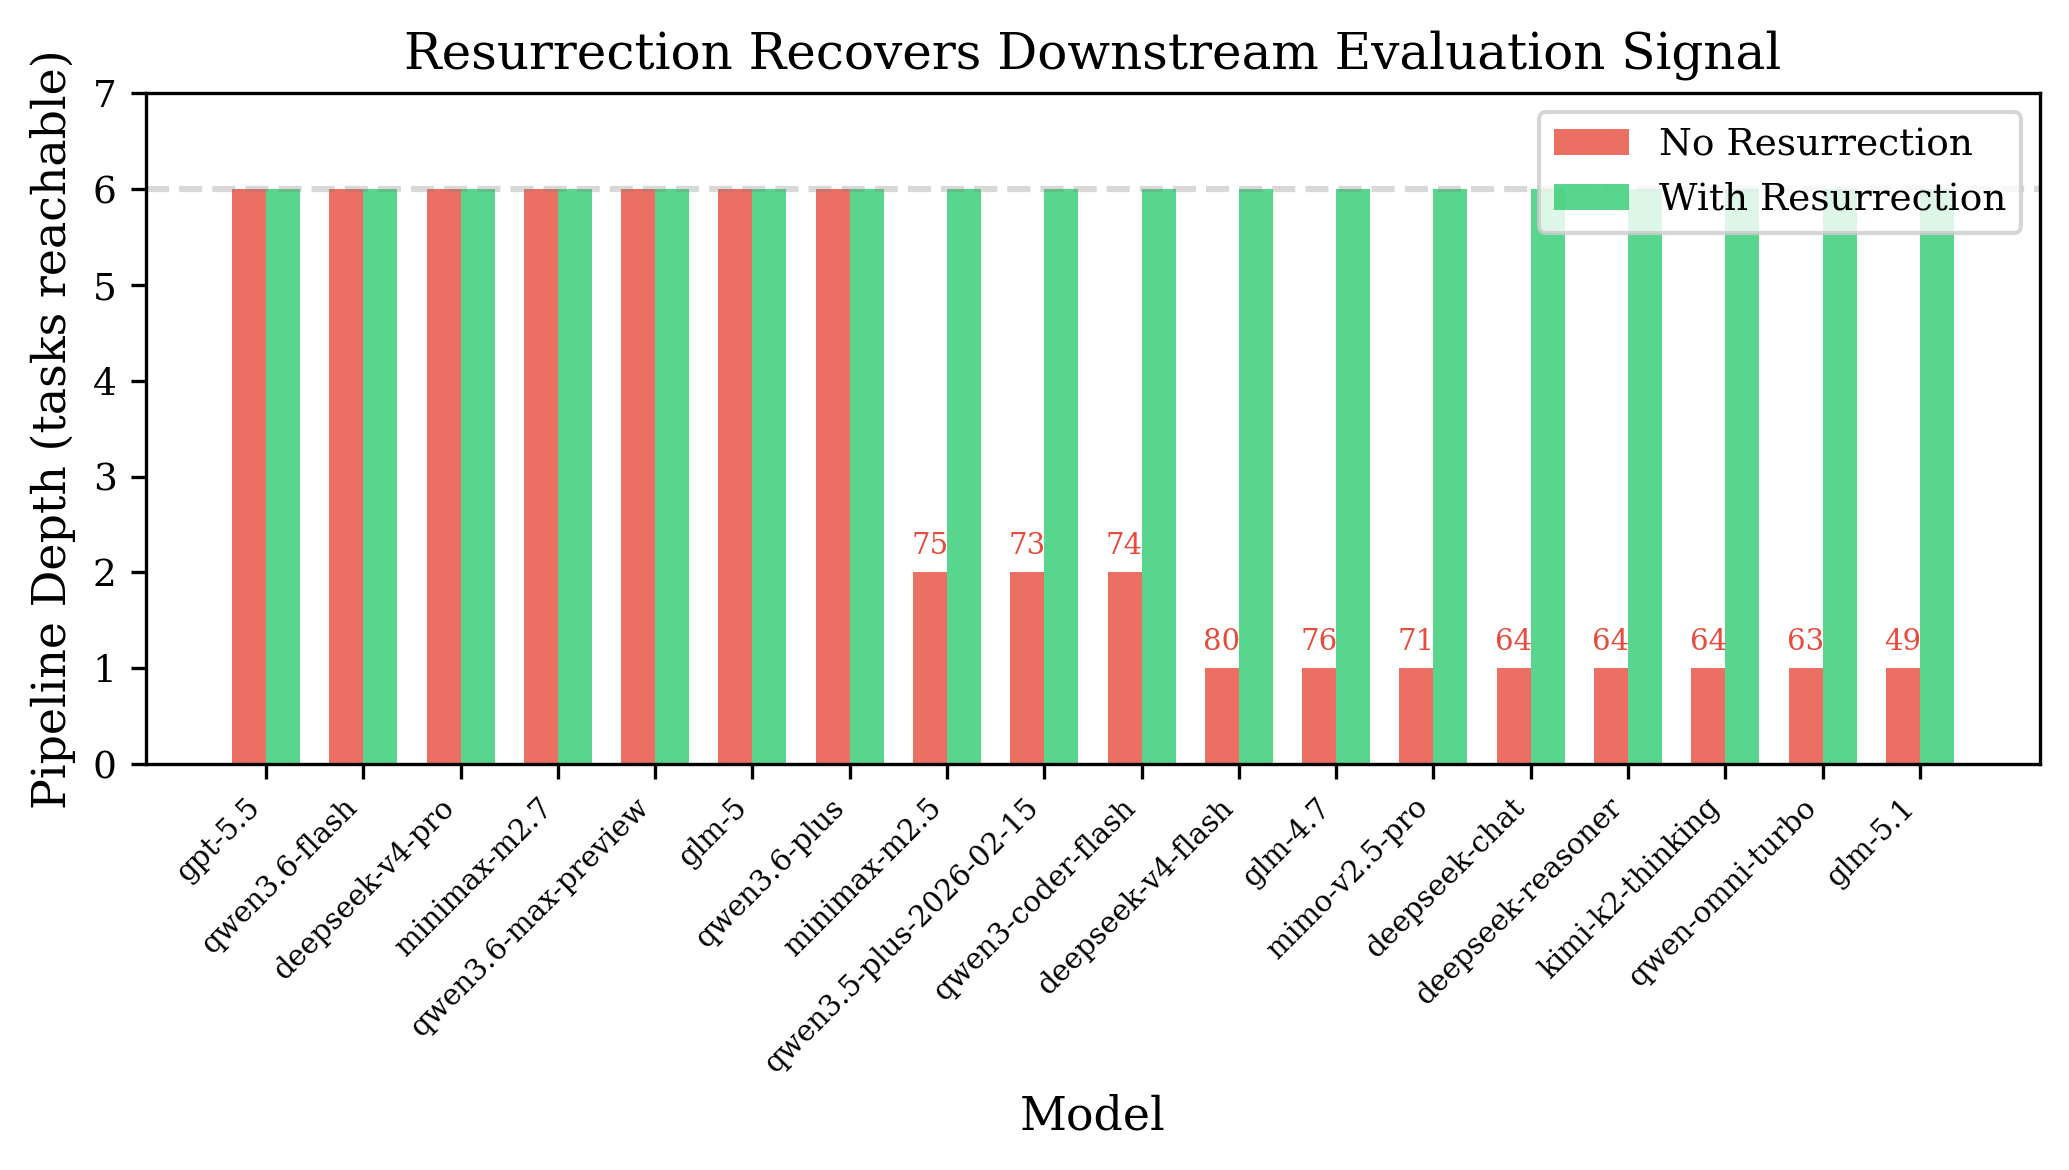
\includegraphics[width=\columnwidth]{figures/fig_resurrection_gain.png}
\caption{Resurrection recovers downstream evaluation signal. Without resurrection, most agents can only be evaluated at 1--2 tasks before cascading failure blocks further measurement. With resurrection, all 6 tasks become reachable, revealing hidden downstream capability.}
\label{fig:resurrection_gain}
\end{figure}

The most striking example is \texttt{claude-sonnet-4.6}: without resurrection, it scores 0 on Tasks~3--5 (pipeline depth = 3, PL = 50.0), but after resurrection at Tasks~2--5, achieves 98.6 on Task~3, 94.6 on Task~4, and 100 on Task~5 (PL = 98.9, MR = 98.3, Rank~2).
This represents a \emph{48.9-point} pipeline score improvement and a jump from Rank~19 to Rank~2---demonstrating that the agent's failure at Task~2 was purely a predecessor effect, not downstream incapability.
Similarly, \texttt{deepseek-v4-flash} scores 0 on Task~1 without resurrection (making Tasks~2--5 unreachable), but after resurrection achieves 100 on Task~2, 93.2 on Task~3, and 89.5 on Task~4.

\textbf{Diagnostic value.}
Without resurrection, the benchmark can only report ``failed at Task~2, pipeline depth = 3.''
With resurrection, it can additionally report ``capable at Tasks~3, 4, 5 given correct parser output,'' providing actionable diagnostic information about \emph{where} the agent's capabilities lie along the dependency chain.

\textbf{Systematic analysis.}
The resurrection gain is not limited to cherry-picked examples: 17 out of 19 configurations achieve $>40$-point pipeline score improvement with resurrection, and the median gain is 73.65 points.
Only GPT-5.5/Codex (which passes all tasks without resurrection) shows zero gain.
The mean resurrection gain across all configurations is 71.55 points, demonstrating that cascading failure systematically obscures downstream capability in serial benchmarks---resurrection recovers this lost signal at scale.

\subsection{Serial Evaluation Preserves Overall Ranking but Reveals Specific Failure Patterns}

To test whether serial evaluation provides different information than static evaluation, we define an \emph{independent-task baseline}: for each model, we compute the average of per-task scores obtained \emph{with resurrection} (i.e., with golden prerequisites provided at each task), which measures each task's capability in isolation.
This baseline represents what a static, independent-task benchmark would report---the agent's per-task competence without serial dependency effects.

We then compare the \emph{no-resurrection serial ranking} (pipeline depth: how far the agent progresses without external correction) against the \emph{independent-task ranking} (average per-task score with golden prerequisites).
A Kendall $\tau$ correlation of 0.763 ($p < 0.001$) confirms that the two rankings are \emph{strongly correlated}---serial evaluation does not wholesale reorder the leaderboard.
However, $\tau = 0.763$ is not 1.0: specific models experience large directional shifts that are invisible in aggregate correlation statistics.

\begin{figure}[t]
\centering

\includegraphics[width=\columnwidth]{figures/fig_score_heatmap.png}
\caption{Per-task score matrix across 18 configurations. The heatmap reveals distinct failure patterns: some models fail at early tasks (T1/T2) while others fail at later tasks (T4), demonstrating that serial evaluation captures qualitatively different information than independent-task benchmarks.}
\label{fig:ranking_shift}
\end{figure}

The most dramatic rank shifts occur for models that fail at early tasks but demonstrate strong downstream capability:
\texttt{deepseek-v4-flash} drops from independent-task rank~8 to no-resurrection rank~14 (shift of 6 positions), because its Task~1 failure blocks the entire pipeline despite achieving 93.2\% on Task~3 and 89.5\% on Task~4 with resurrection.
Similarly, \texttt{glm-4.7} shifts 5 positions (rank~9 $\to$ rank~14).
These shifts are not artifacts---they reflect the real-world consequence of serial dependency: an agent that cannot produce a working lexer \emph{cannot} demonstrate its parser or optimizer capability in a serial workflow, regardless of how capable those downstream components are.

A Wilcoxon signed-rank test on the paired rank differences yields $W = 34.5$, $p = 0.44$, indicating that the \emph{overall} ranking structure is preserved (consistent with the high Kendall $\tau$), but individual models can experience large directional shifts.
The key finding is not that serial evaluation \emph{reorders} the entire ranking, but that it \emph{selectively penalizes} models with early-stage failures while \emph{rewarding} those with consistent cross-task continuity---a qualitative distinction that Kendall $\tau$ alone cannot capture.
This result supports Hypothesis~H1: serial benchmarks measure a distinct evaluation axis that static benchmarks do not capture.

\subsection{Model--Scaffold Interaction}

The choice of agent scaffold significantly affects outcomes.
The same model (\texttt{mimo-v2.5-pro}) scores 67.04 on OpenHands versus 98.23 on Kimi CLI---a 31-point gap attributable entirely to scaffold design differences in action space, retry logic, and context management.
Among OpenHands-based configurations, the same scaffold produces widely varying results across models, confirming that \emph{model strength alone does not determine agent performance}---the scaffold is an independent variable that must be controlled and reported in evaluation frameworks.

\subsection{\yatcc{} vs. \yatcc{}-Hard: The Scaffolding Gap}

Table~\ref{tab:hard} presents the \yatcc{}-Hard leaderboard across 18 model configurations.
The difficulty gap between the two workloads quantifies the value of scaffolding in agentic coding tasks.

\begin{table}[t]
\centering
\small
\begin{tabular}{lrrrrrrrr}
\toprule
\textbf{Model} & \textbf{T0} & \textbf{T1} & \textbf{T2} & \textbf{T3} & \textbf{T4} & \textbf{T5} & \textbf{PL} & \textbf{Res} \\
\midrule
qwen3.6-max-preview & 100 & 100 & 86.0 & 86.3 & 94.5 & 100 & 94.5 & 0 \\
deepseek-v4-pro & 100 & 100 & 79.5 & 87.7 & 66.5 & 98.4 & 88.7 & 1 \\
glm-5.1 & 100 & 100 & 89.1 & 91.8 & 42.8 & 100 & 87.3 & 2 \\
deepseek-v4-flash & 100 & 100 & 77.8 & 89.0 & 61.1 & 60.9 & 81.5 & 0 \\
qwen3.6-plus & 100 & 100 & 77.1 & 19.2 & 67.3 & 96.9 & 76.7 & 2 \\
glm-5 & 100 & 100 & 65.7 & 65.8 & 66.4 & 50.0 & 74.6 & 2 \\
minimax-m2.7 & 100 & 80.4 & 33.5 & 41.1 & 66.1 & 60.9 & 63.7 & 2 \\
kimi-k2.6 & 100 & 100 & 18.0 & 41.1 & 55.2 & 75.0 & 64.9 & 3 \\
\bottomrule
\end{tabular}
\caption{\yatcc{}-Hard leaderboard (top 8 of 18). Scores drop significantly compared to \yatcc{}---the best model achieves only PL=94.5 on Hard vs.\ PL=99.3 on \yatcc{}.}
\label{tab:hard}
\end{table}

\textbf{Key observation.}
The best \yatcc{}-Hard score (PL=94.5 by \texttt{qwen3.6-max-preview}) is 4.8 points below the best \yatcc{} score (PL=99.3 by \texttt{kimi-k2.6}).
More dramatically, models that excel on \yatcc{} often collapse on \yatcc{}-Hard: \texttt{kimi-k2.6} drops from PL=99.3 (Rank~1 on \yatcc{}) to PL=64.9 (Rank~8 on \yatcc{}-Hard), a 34.4-point decline.
This gap reveals that scaffolded starter code provides substantial leverage---models that appear capable when filling in blanks may lack the architectural reasoning required for full from-scratch implementation.

The resurrection mechanism is equally critical on \yatcc{}-Hard: 12 out of 18 configurations require at least one resurrection, and the median resurrection gain is comparable to \yatcc{}.
This confirms that cascading failure is a workload-independent phenomenon---it affects both scaffolded and from-scratch settings, and resurrection provides diagnostic value in both contexts.